\documentclass[12pt,a4paper]{ctexart}
\usepackage[margin=2.2cm]{geometry}
\usepackage{graphicx}
\usepackage{booktabs}
\usepackage{amsmath}
\usepackage{float}
\usepackage{hyperref}
\usepackage{xcolor}
\usepackage{listings}

\lstset{
  language=C,
  basicstyle=\ttfamily\small,
  keywordstyle=\color{blue!70!black},
  commentstyle=\color{green!40!black},
  stringstyle=\color{orange!60!black},
  showstringspaces=false,
  breaklines=true,
  frame=single,
  tabsize=4
}

% ===== 实验信息 =====
\newcommand{\reporttitle}{DFA 运行模拟实验报告}
\newcommand{\subtask}{DFA 输入、检查、枚举与判定}
\newcommand{\authname}{姓名}
\newcommand{\authid}{学号}
% =====================

\title{\reporttitle}
\author{\authname：\underline{\hspace{3cm}} \quad \authid：\underline{\hspace{3cm}}}
\date{\today}

\begin{document}
\maketitle

\section{实验目的}
本实验围绕有限自动机 DFA 的运行过程展开，目标如下：
\begin{itemize}
  \item 理解 DFA 的五元组表示方法，以及字符集、状态集、初态、终态和转移函数之间的关系。
  \item 使用 C 语言实现 DFA 的输入、存储、合法性检查与运行模拟。
  \item 实现语言枚举和字符串判定功能，验证 DFA 对输入串的接受与拒绝过程。
\end{itemize}

\section{实验过程}
\subsection{实验环境}
\begin{itemize}
  \item 操作系统：macOS
  \item 编程语言：C
  \item 编译器：gcc / clang
  \item 其他工具：LaTeX，VS Code
\end{itemize}

\subsection{数据集与预处理}
本实验不依赖外部数据集，DFA 的输入保存在文本文件中。当前示例文件为 \texttt{dfa\_in1.dfa}，其结构为：
\begin{itemize}
  \item 第 1 行：字符集，例如 \texttt{ab}
  \item 第 2 行：状态总数，例如 \texttt{4}
  \item 第 3 行：开始状态
  \item 第 4 行：接受状态集
  \item 第 5 行及之后：每个状态在字符集各符号上的转移结果
\end{itemize}

程序在加载文件后，会对以下内容进行检查：开始状态是否在状态范围内、接受状态集是否非空、转移是否越界、字符集是否存在重复符号。

\subsection{实现步骤}
\begin{enumerate}
  \item 读取 DFA 文本文件，解析字符集、状态信息和转移表，并存入结构体。
  \item 对 DFA 合法性进行检查，防止无效自动机参与后续模拟。
  \item 设计字符串模拟过程，从初态开始沿着转移表逐字符推进，输出中间状态变化。
  \item 实现长度上界枚举与随机字符串判定，分别对应语言输出与规则判定功能。
\end{enumerate}

\section{实验内容}
\subsection{任务一：DFA 输入与合法性检查}
程序首先读取 \texttt{dfa\_in1.dfa}，将字符集、状态数、开始状态、接受状态和转移表保存到内存中。对于输入文件，程序采用逐行读取方式，跳过空行并解析整数，避免格式错误影响运行。

主要检查点如下：
\begin{itemize}
  \item 字符集不能为空，且不能出现重复符号。
  \item 开始状态必须位于 $[1, n]$ 内。
  \item 接受状态集不能为空。
  \item 每个状态对每个字符都必须给出合法的下一状态。
\end{itemize}

\subsection{任务二：DFA 运行模拟与字符串判定}
字符串判定时，程序从开始状态出发，按输入串逐字符查询转移表并更新当前状态。若输入字符不属于字符集，程序立即判为拒绝。输入结束后，根据当前状态是否属于接受状态集，给出接受或拒绝结论。

随机判定功能则先根据字符集随机生成一个指定长度的字符串，再调用同样的模拟过程，保证判定逻辑统一。

\subsection{任务三：长度不超过 $N$ 的语言枚举}
当用户输入最大长度 $N$ 后，程序通过递归遍历字符集构造所有长度不超过 $N$ 的字符串，并逐个调用模拟过程判断是否被接受。若字符串被接受，则输出该串；空串用 \texttt{<epsilon>} 表示。

该方法适合实验规模较小的 DFA，可直接展示语言的部分成员集合，便于人工检查转移逻辑是否正确。

\section{实验结果}
\subsection{任务一结果：程序启动与 DFA 加载}
程序启动后会自动尝试加载默认文件 \texttt{dfa\_in1.dfa}，结果如图~\ref{fig:init} 所示。

\begin{figure}[H]
\centering
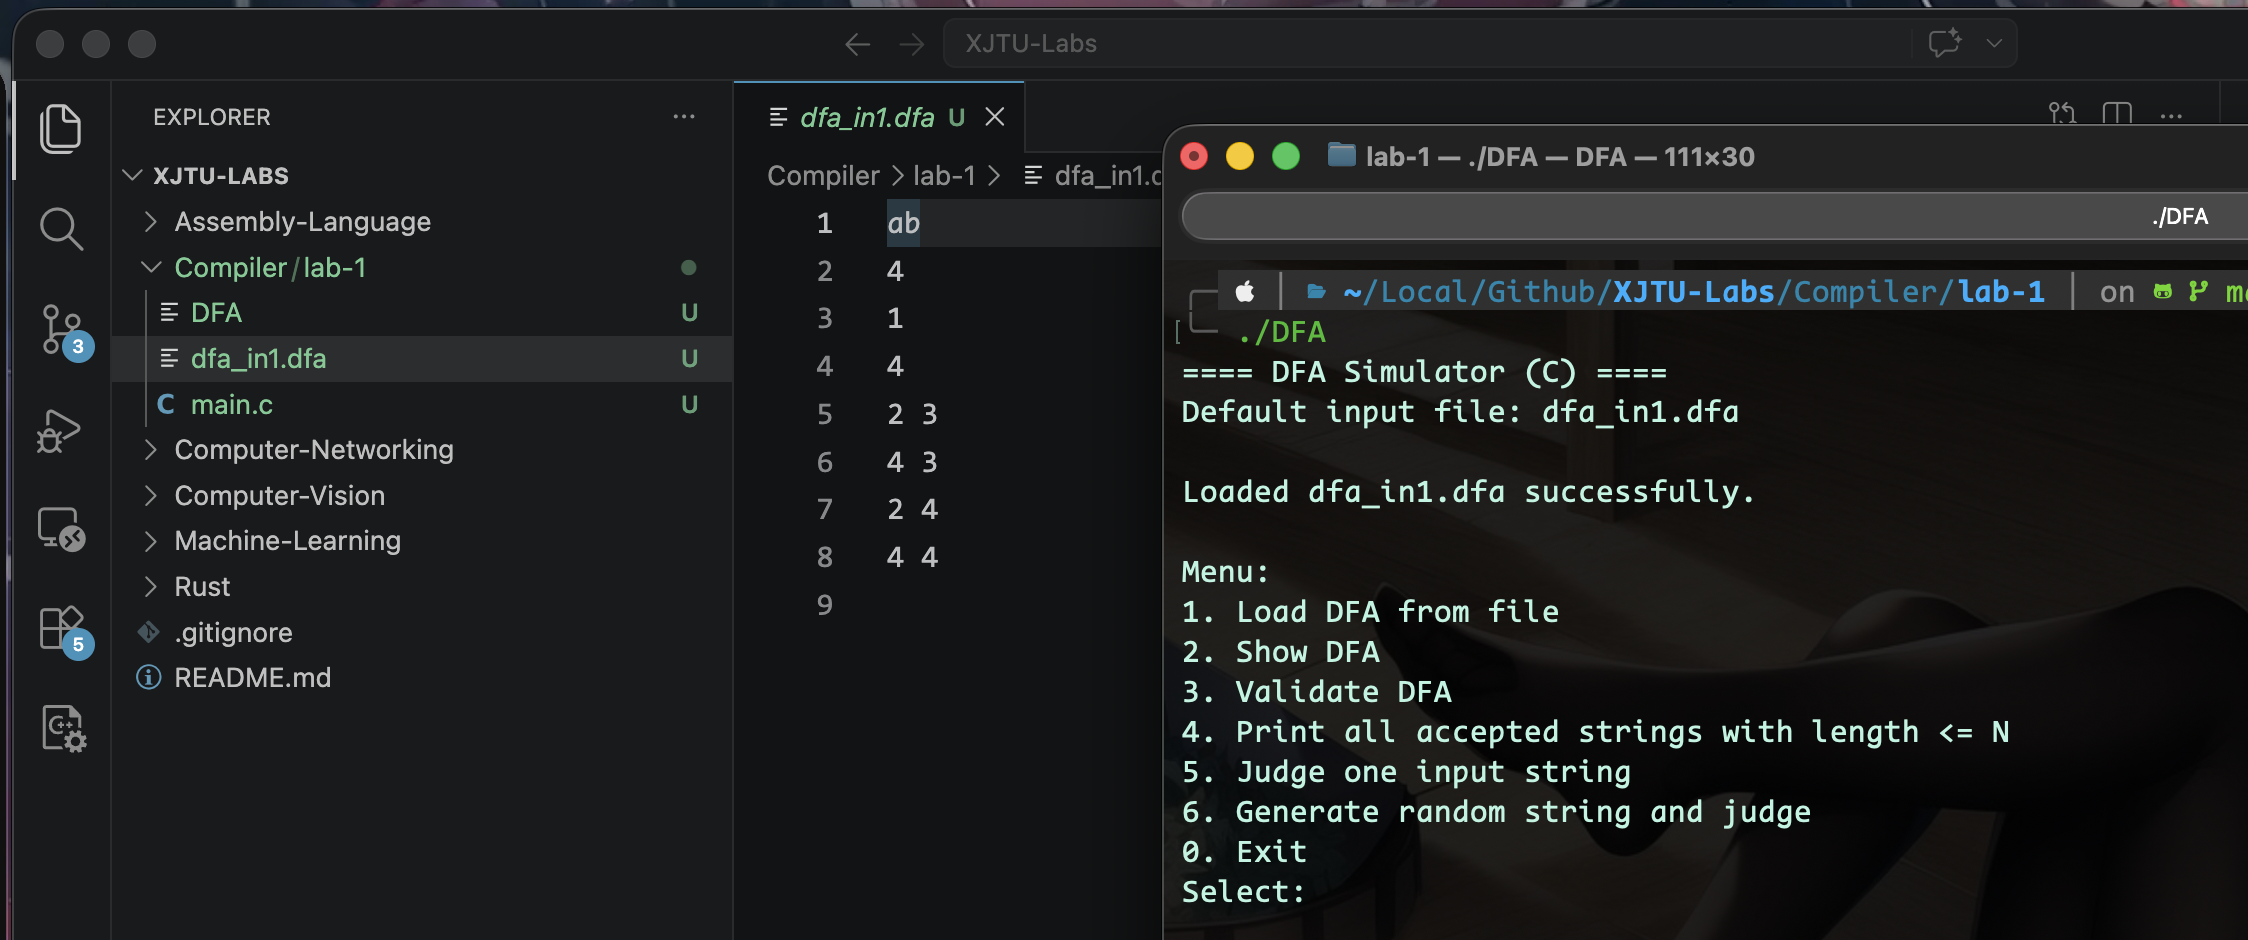
\includegraphics[width=0.95\textwidth]{../results/init.png}
\caption{程序初始化与默认 DFA 加载结果}
\label{fig:init}
\end{figure}

结果分析：
\begin{itemize}
  \item 默认文件能够正常读取，说明文本解析流程正确。
  \item 菜单化交互方便后续切换查看 DFA、枚举语言和判定字符串。
\end{itemize}

\subsection{任务二结果：DFA 转移表展示}
选择“Show DFA”后，程序会输出字符集、状态范围、开始状态、接受状态及每个状态的转移表，如图~\ref{fig:table} 所示。

\begin{figure}[H]
\centering
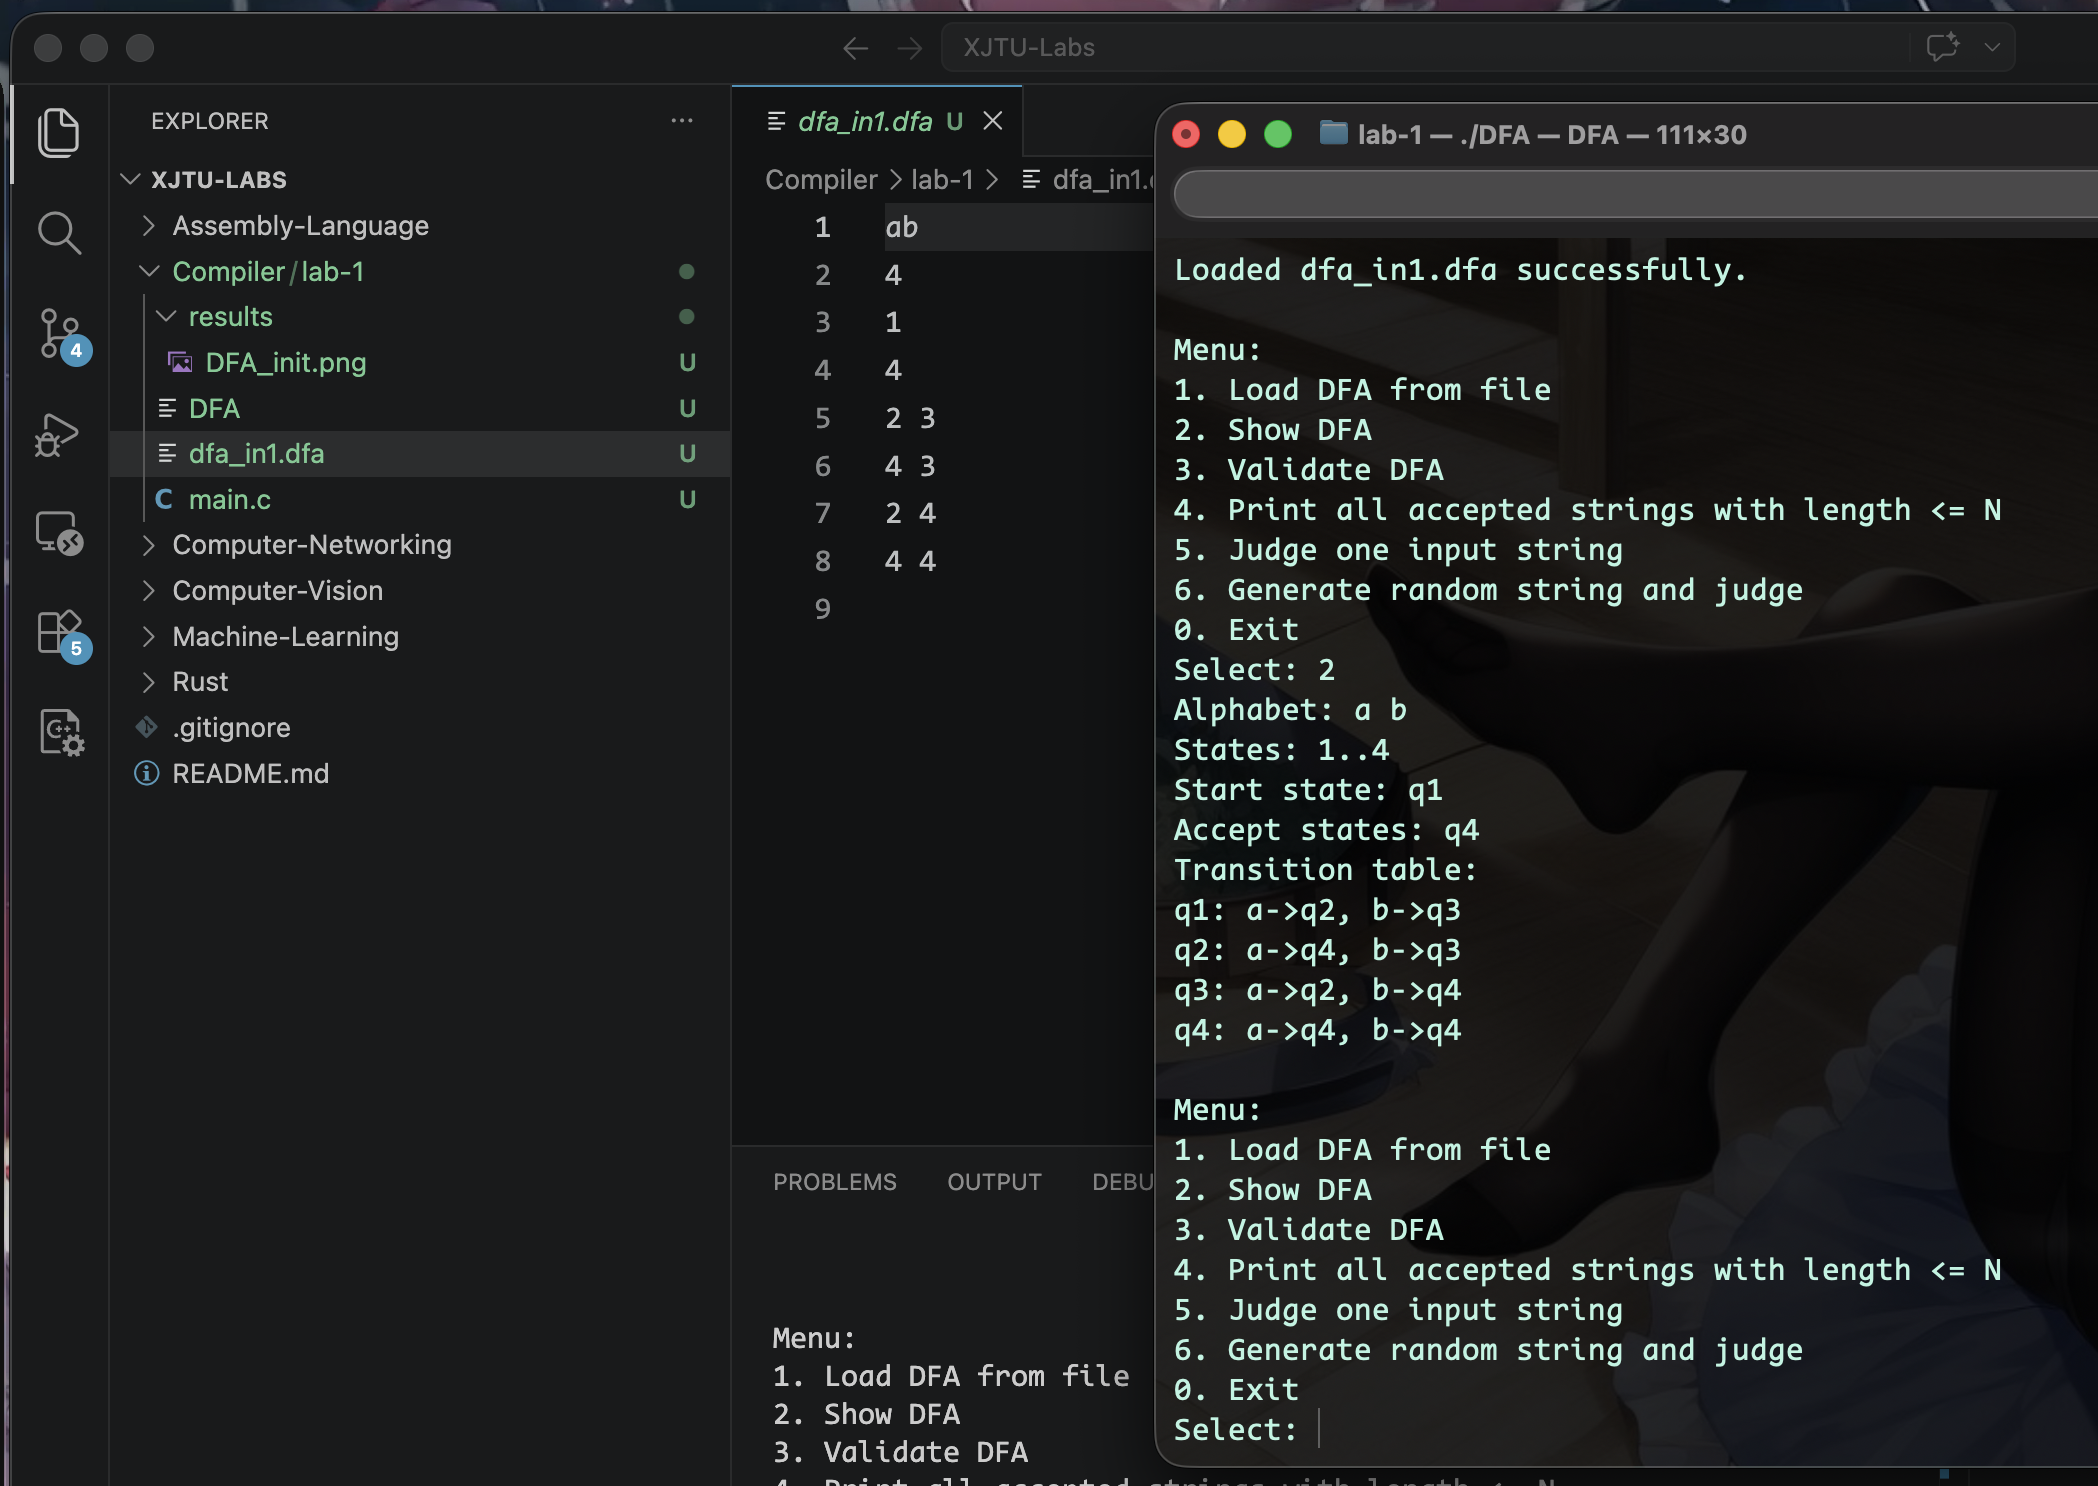
\includegraphics[width=0.95\textwidth]{../results/transition_table.png}
\caption{DFA 转移表与基本信息输出}
\label{fig:table}
\end{figure}

结果分析：
\begin{itemize}
  \item 转移表可以清楚显示每个输入符号对应的下一状态。
  \item 该输出有助于对照实验文件，检查 DFA 定义是否与预期一致。
\end{itemize}

\subsection{任务三结果：长度不超过 $N$ 的串输出}
在输入最大长度 $N=2$ 后，程序枚举出该 DFA 语言中长度不超过 2 的所有字符串，如图~\ref{fig:maxlen} 所示。

\begin{figure}[H]
\centering
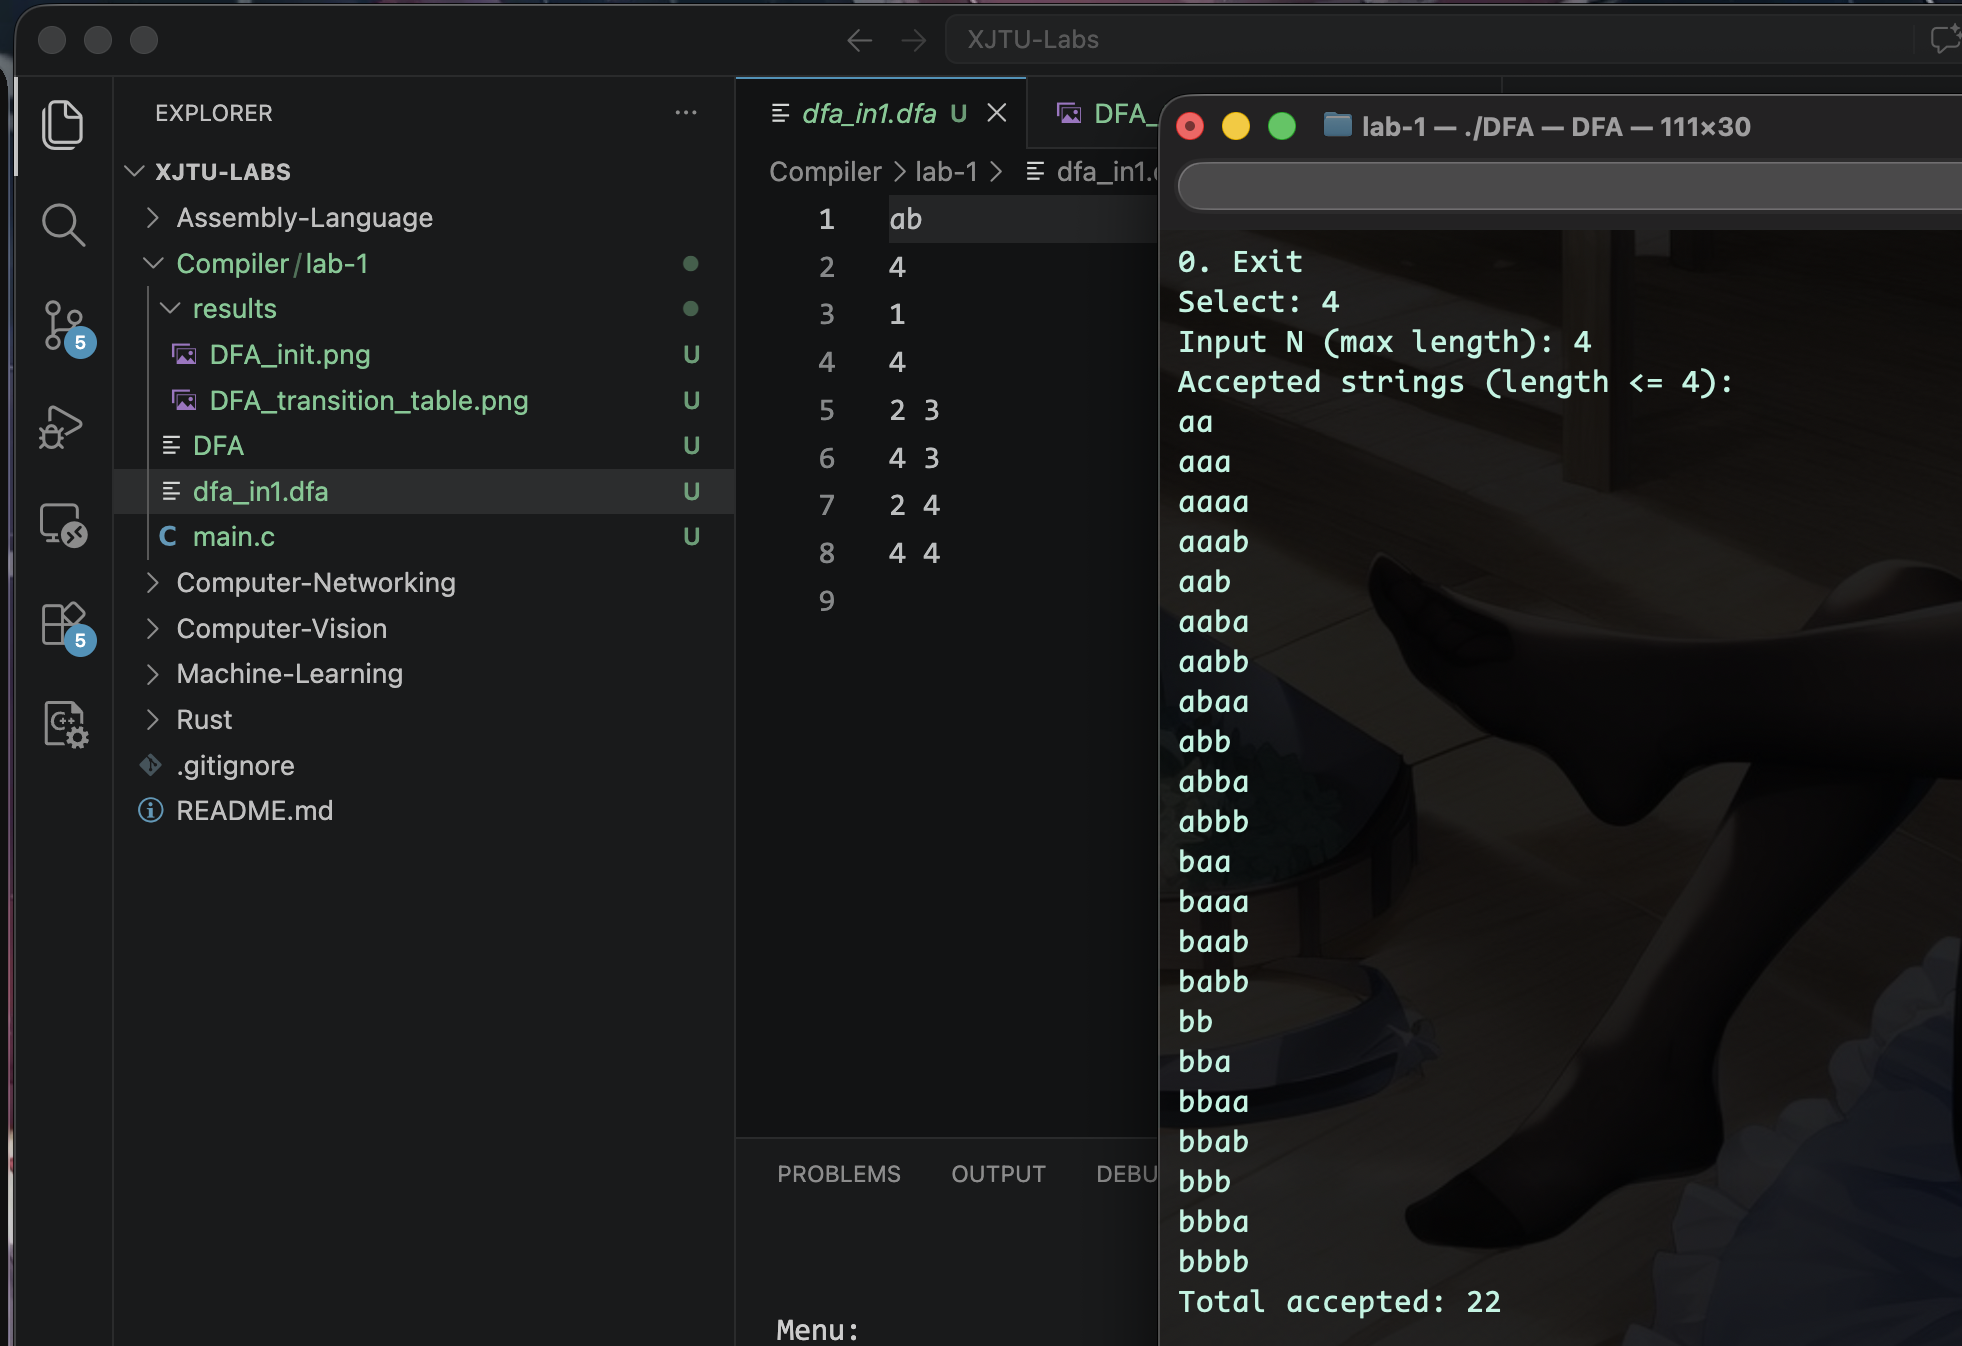
\includegraphics[width=0.95\textwidth]{../results/max_length_output.png}
\caption{长度不超过 $N$ 的接受串输出}
\label{fig:maxlen}
\end{figure}

结果分析：
\begin{itemize}
  \item 枚举结果能够体现 DFA 的语言成员结构。
  \item 通过该输出可以快速验证转移关系与接受状态设置是否合理。
\end{itemize}

\subsection{任务四结果：字符串判定}
程序对输入串进行逐步模拟，并输出状态变化过程，如图~\ref{fig:judge} 所示。

\begin{figure}[H]
\centering
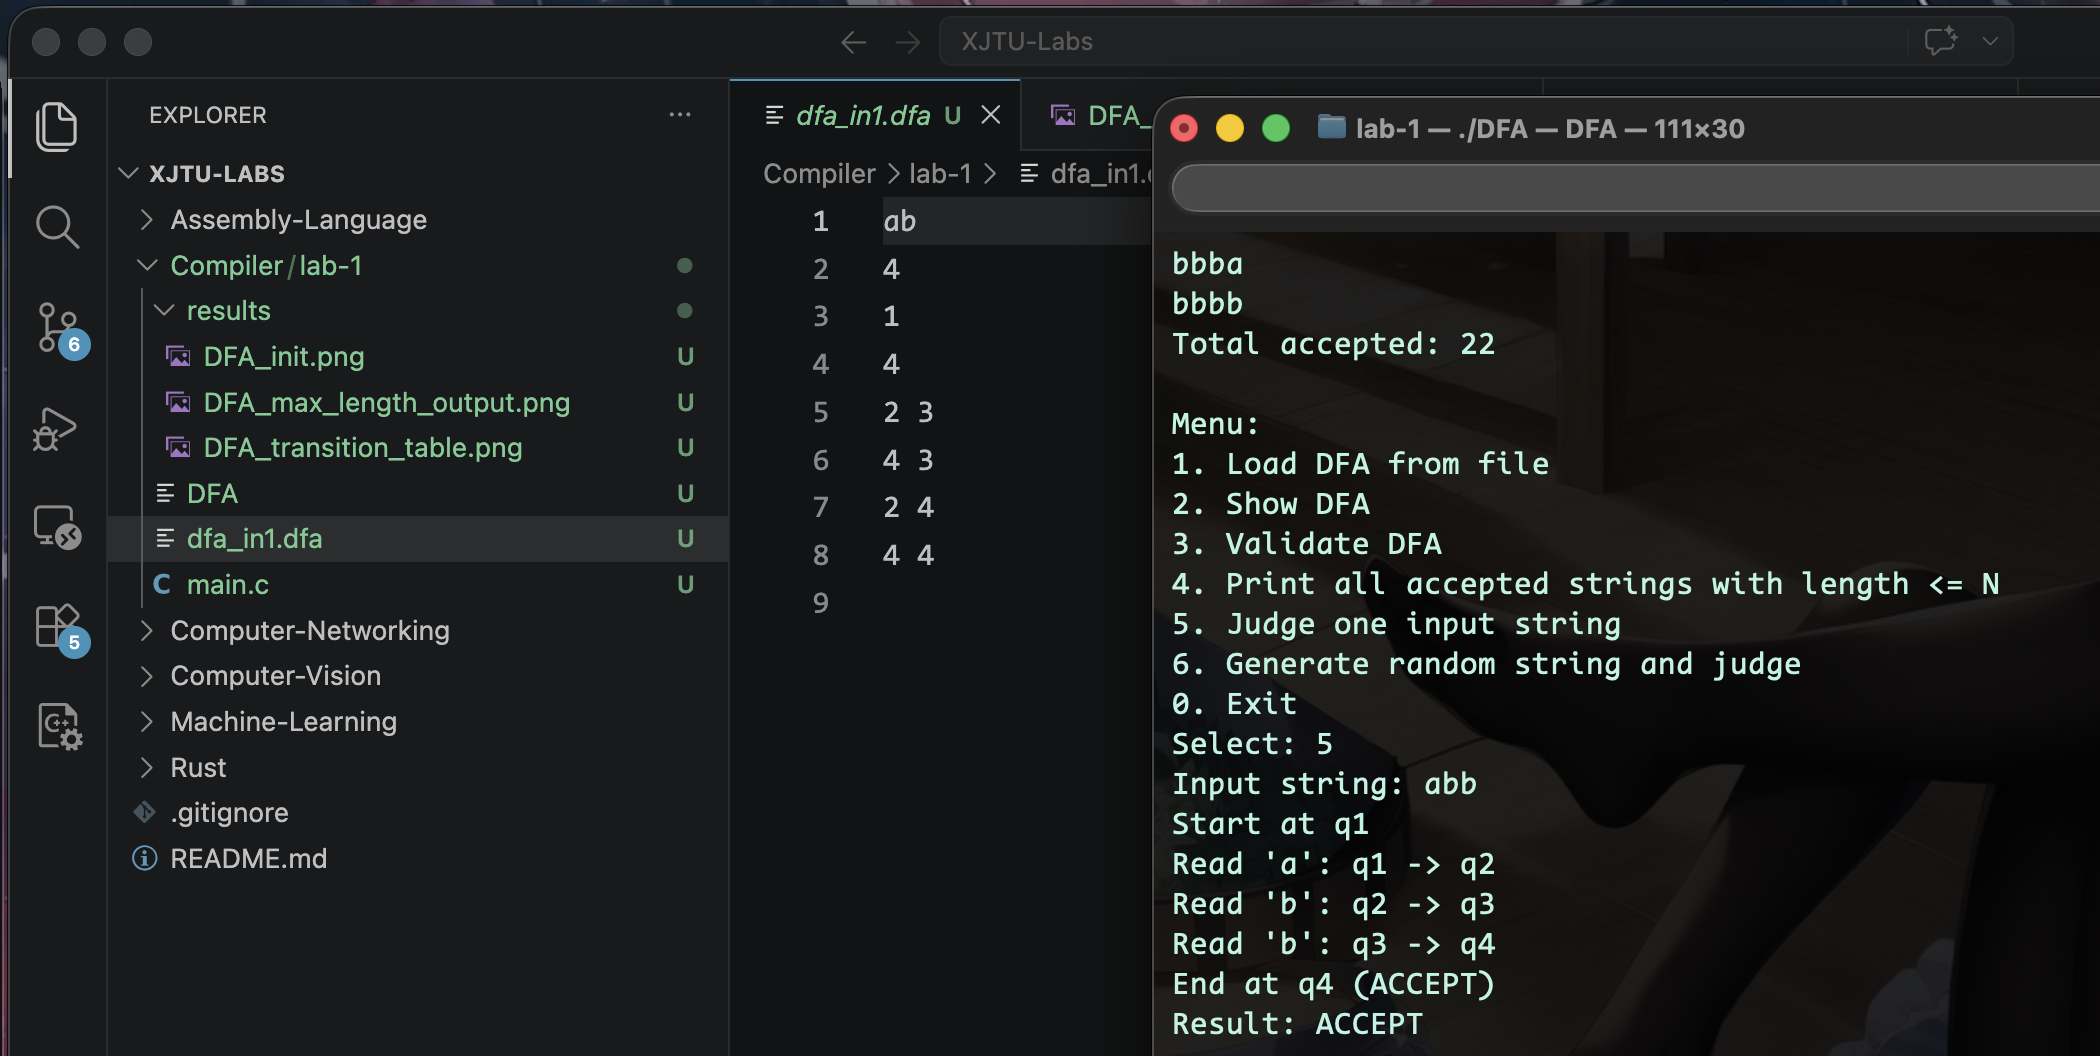
\includegraphics[width=0.95\textwidth]{../results/input_string_result.png}
\caption{输入字符串的 DFA 判定过程}
\label{fig:judge}
\end{figure}

结果分析：
\begin{itemize}
  \item 模拟过程直观展示了从开始状态到最终状态的迁移路径。
  \item 该结果可用于验证某个字符串是否属于 DFA 语言。
\end{itemize}

\section{总结}
本实验完成了 DFA 模拟程序的核心功能，包括文本输入、合法性检查、语言枚举与字符串判定：
\begin{itemize}
  \item 完成了 DFA 五元组的文件读取与结构化存储。
  \item 实现了 DFA 合法性检查，能够发现明显的输入错误。
  \item 实现了字符串模拟、长度限制枚举和随机字符串判定功能。
\end{itemize}

通过本实验，对 DFA 的形式化定义和运行机制有了更直观的理解，也加深了对自动机状态迁移过程的认识。

\section*{附录：实验源代码}
\subsection*{A.1 主要源码：main.c}
\lstinputlisting{../main.c}

\subsection*{A.2 运行命令}
\begin{verbatim}
cd /Users/rinalic/Local/Github/XJTU-Labs/Compiler/lab-1
gcc -std=c11 -Wall -Wextra -pedantic main.c -o DFA
./DFA
\end{verbatim}

\end{document}
